\chapter{Transmission and detection of a single CDMA signal}

\section{Scenario}
A single transmit signal of a mobile station is transmitted to the base station over the DPCH (up-link).\cite{e1}

\section{Task}
In the experiment we should receive and detect the data symbols from the received signal. Usually there is multi path propagation because of reflections at walls, ceiling etc. However, in our case it is sufficient to implement a simple matched filter receiver. \textcolor{red}{(why???)}

\section{Information about transmit signal}
\begin{itemize}
	\item Signal name: TxSignal\_1.mat \label{siginfo}
	\item Parameter specifications:
\end{itemize}
\begin {table}[H]
\centering
\begin{tabular}{|c|c|}
	
	\hline
	burst type & 1 \\    \hline
	spreading factor & 8 \\   \hline
	number of data symbols per data field & 122 \\   \hline
	channelization code sequence  & $\left[1 1 1 1 1 1 1 1\right]$ \\   \hline
	midamble ID & Basiscode : 1, User : 1 \\   \hline
	scrambling code ID & 1 \\ 
	\hline
\end{tabular}
\caption {Parameters of the transmit signal}
\end{table}

\section{Algorithm description\cite{e1}}
\begin{enumerate}
	\item Transmission of the UMTS signal as described above.
	\item Load the file with the received signal as well as the file with the transmit signal information (\ref{siginfo}) into the Matlab workspace
	\item Select one of the two received signal sample streams: xi = xi(1,:); xq = xq(1,:);
	\item normalize the signal samples to get a convenient range of sample values: xi = xi/$2^{14}$, xq = xq /$2^{14}$
	\item Remove the mean values of vectors xi and xq
	\item Establish a complex signal vector out of the inphase and quadrature components:\\
	x = xi + 1i*xq: or x = complex(xi,xq);
	\item Apply the digital Rx pulse shape filter: x = RxFilter(x);
	\item Cut out the 15 signal bursts which are contained in the time slots of the filtered signal vector. The first time slot begins around sample index 1000, the length of the signal bursts is 10240 samples
	\item The code sequences "midamble", "code", "scr" contain one element per signal chip. To use these sequences for signal processing they have to match our oversampling of eight samples per chip. We do the fitting by so called "zero stuffing" of the code sequence vectors by means of the Kronecker product.
	\item The next steps have to be done in a loop for every signal burst:
	\begin{enumerate}[label = (\alph*)]
		\item Remove the mean value from the burst signal
		\item Increase the sample time resolution by signal interpolation
		\item Calculate the cross correlation function of the up-sampled signal burst with the zero-stuffed mid-amble sequence
		\item Search the position of the maximum absolute value of the cross correlation vector
		\item Cut out the signal samples of the first data part of the signal burst
		\item Cut out the signal samples of the second data part of the signal burst
		\item Correct the signal phase rotation by multiplying the data part vectors by the complex conjugate value of the cross correlation value at vector index Imax
		\item De-scramble the data parts by using "descramble()"
		\item De-spread the data parts by using "despread()"
		\item Decide the data symbols by using "decide()"
		\item Determine and count the number of data symbol detection errors
	\end{enumerate}
\end{enumerate}

\section{Observation and interpretation}
\begin{figure}[H]
	\begin{center}
		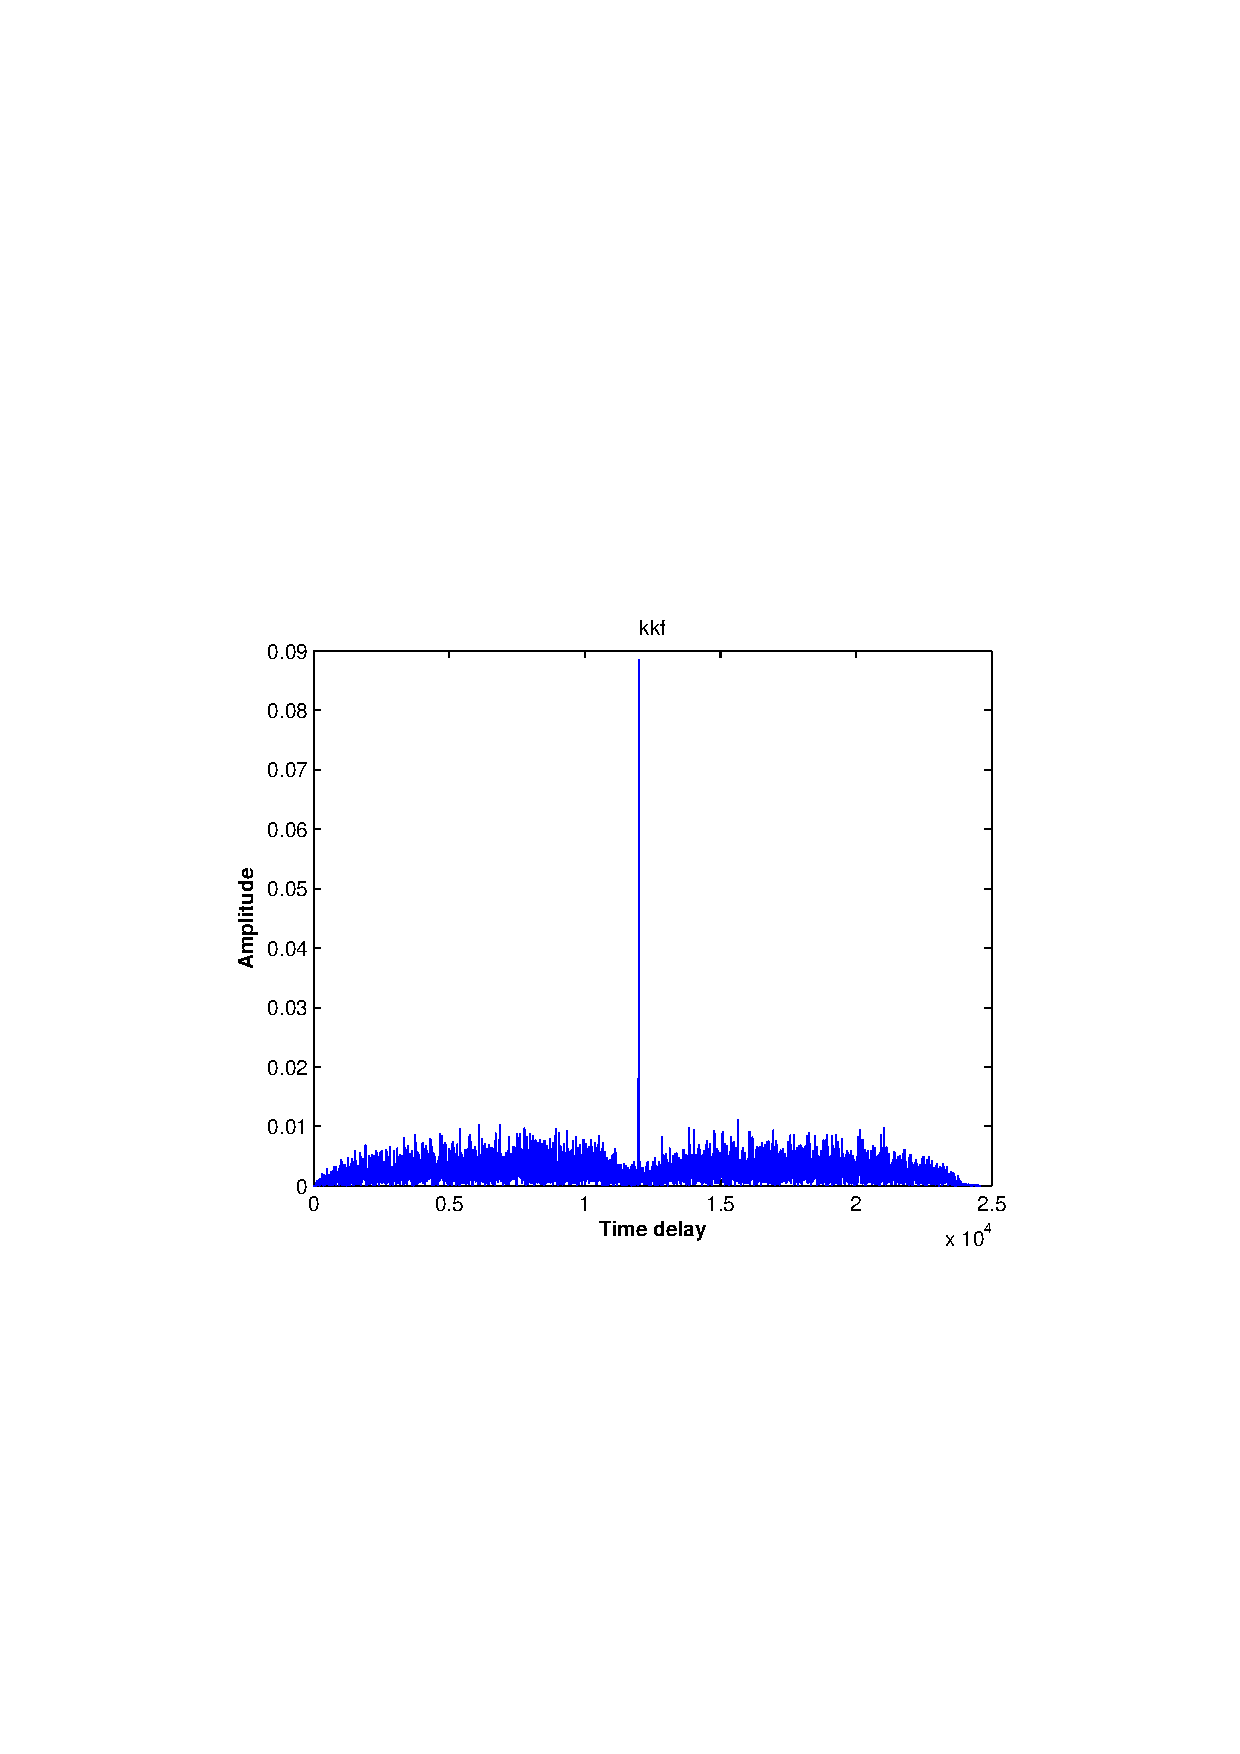
\includegraphics[scale=0.5]{ex1/kkf.pdf}
		\caption{Cross correlation function}
		\label{kkf}
	\end{center}
\end{figure}
The operation of KKF can get rid of the time delay in the channel. In figure \ref{kkf} we can see there is a peak with index Imax. This is the position of last midamble bit. After detecting the Imax we can cut out the first and the second part of the data from the following positions:

The first part start index: $Imax - (976 + 512)*8 +1 = Imax - 11903$, length: $976*8 = 7808$

The second part start index: $Imax+1$, length: $976*8 = 7808$

After the operation of  phase rotation we can get figure \ref{fig:ex1:beDescr}. It is hard to recognize them with respect to the original QPSK data. After the operation of descramble, we can plot the data like figure \ref{fig:ex1:aftdescr}. Furthermore, after the operation of despread we get data as shown in figure \ref{fig:ex1:aftdespr}. Then, we can simply use the decide function to decide the final data.
\begin{figure}[H]
	\begin{center}
		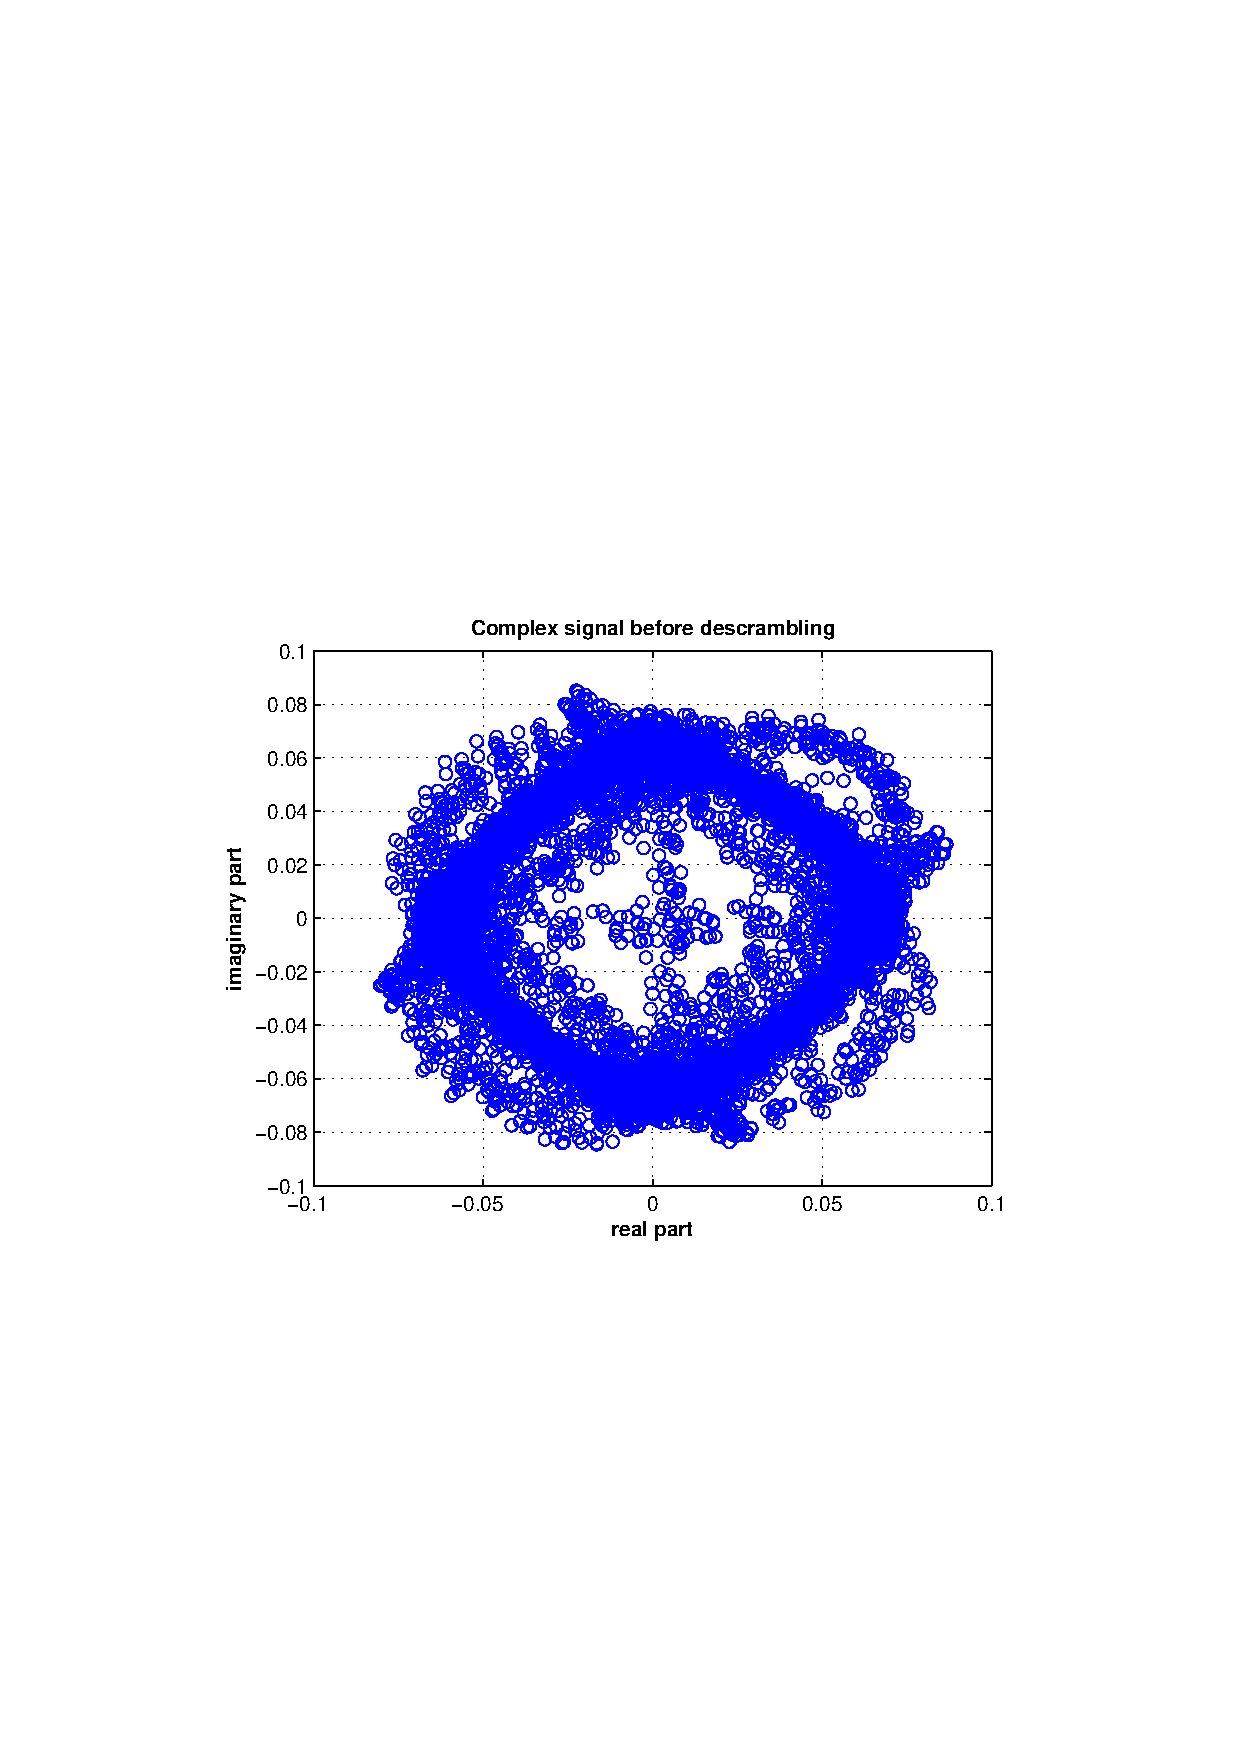
\includegraphics[scale=0.5]{ex1/beforeDescramble.pdf}
		\caption{Complex signal before descrambling}
		\label{fig:ex1:beDescr}
	\end{center}
\end{figure} 

\begin{figure}[H]
	\begin{center}
		\subfigure[after descramble]{\label{fig:ex1:aftdescr}
			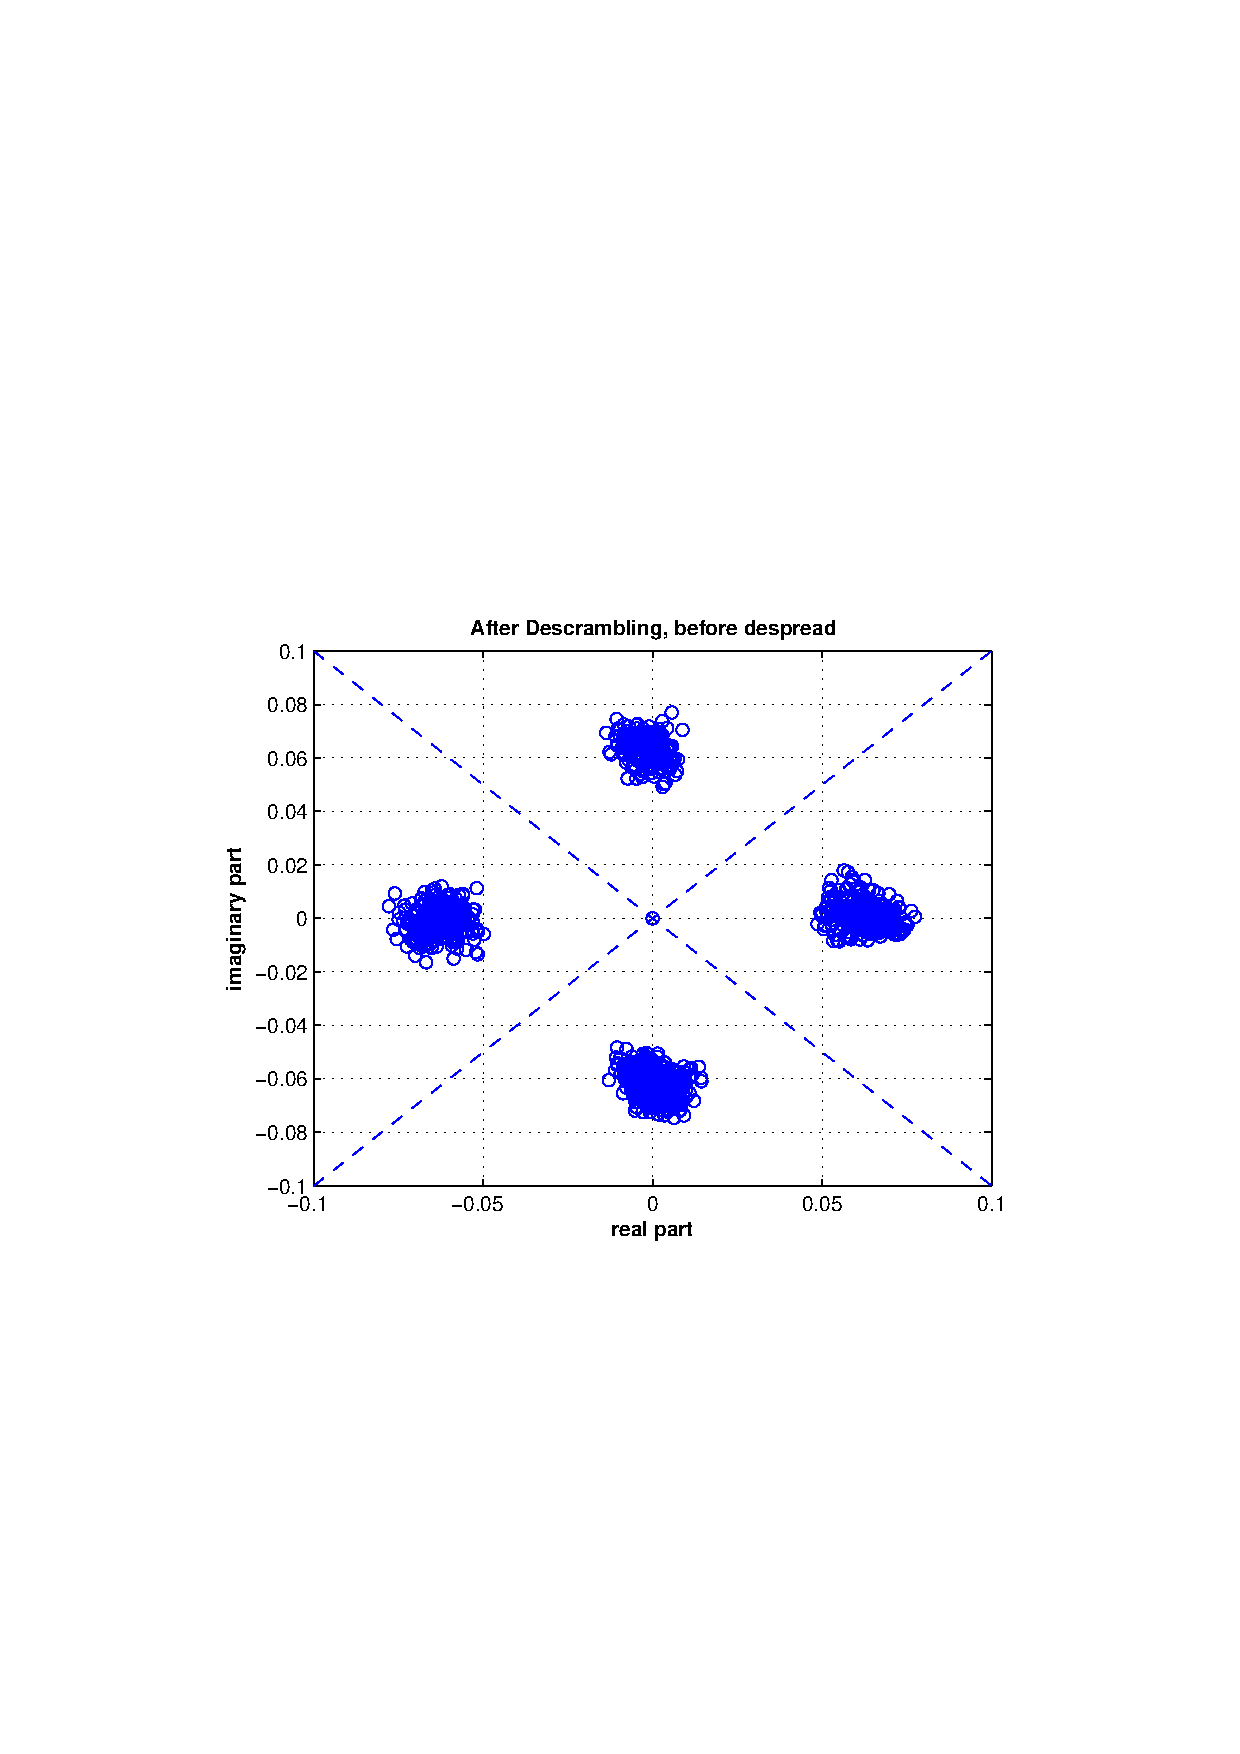
\includegraphics[width=3in]{ex1/afterDescramble.pdf} }
		\hspace{1in} %\vspace{x mm}
		\subfigure[after despread]{\label{fig:ex1:aftdespr}
			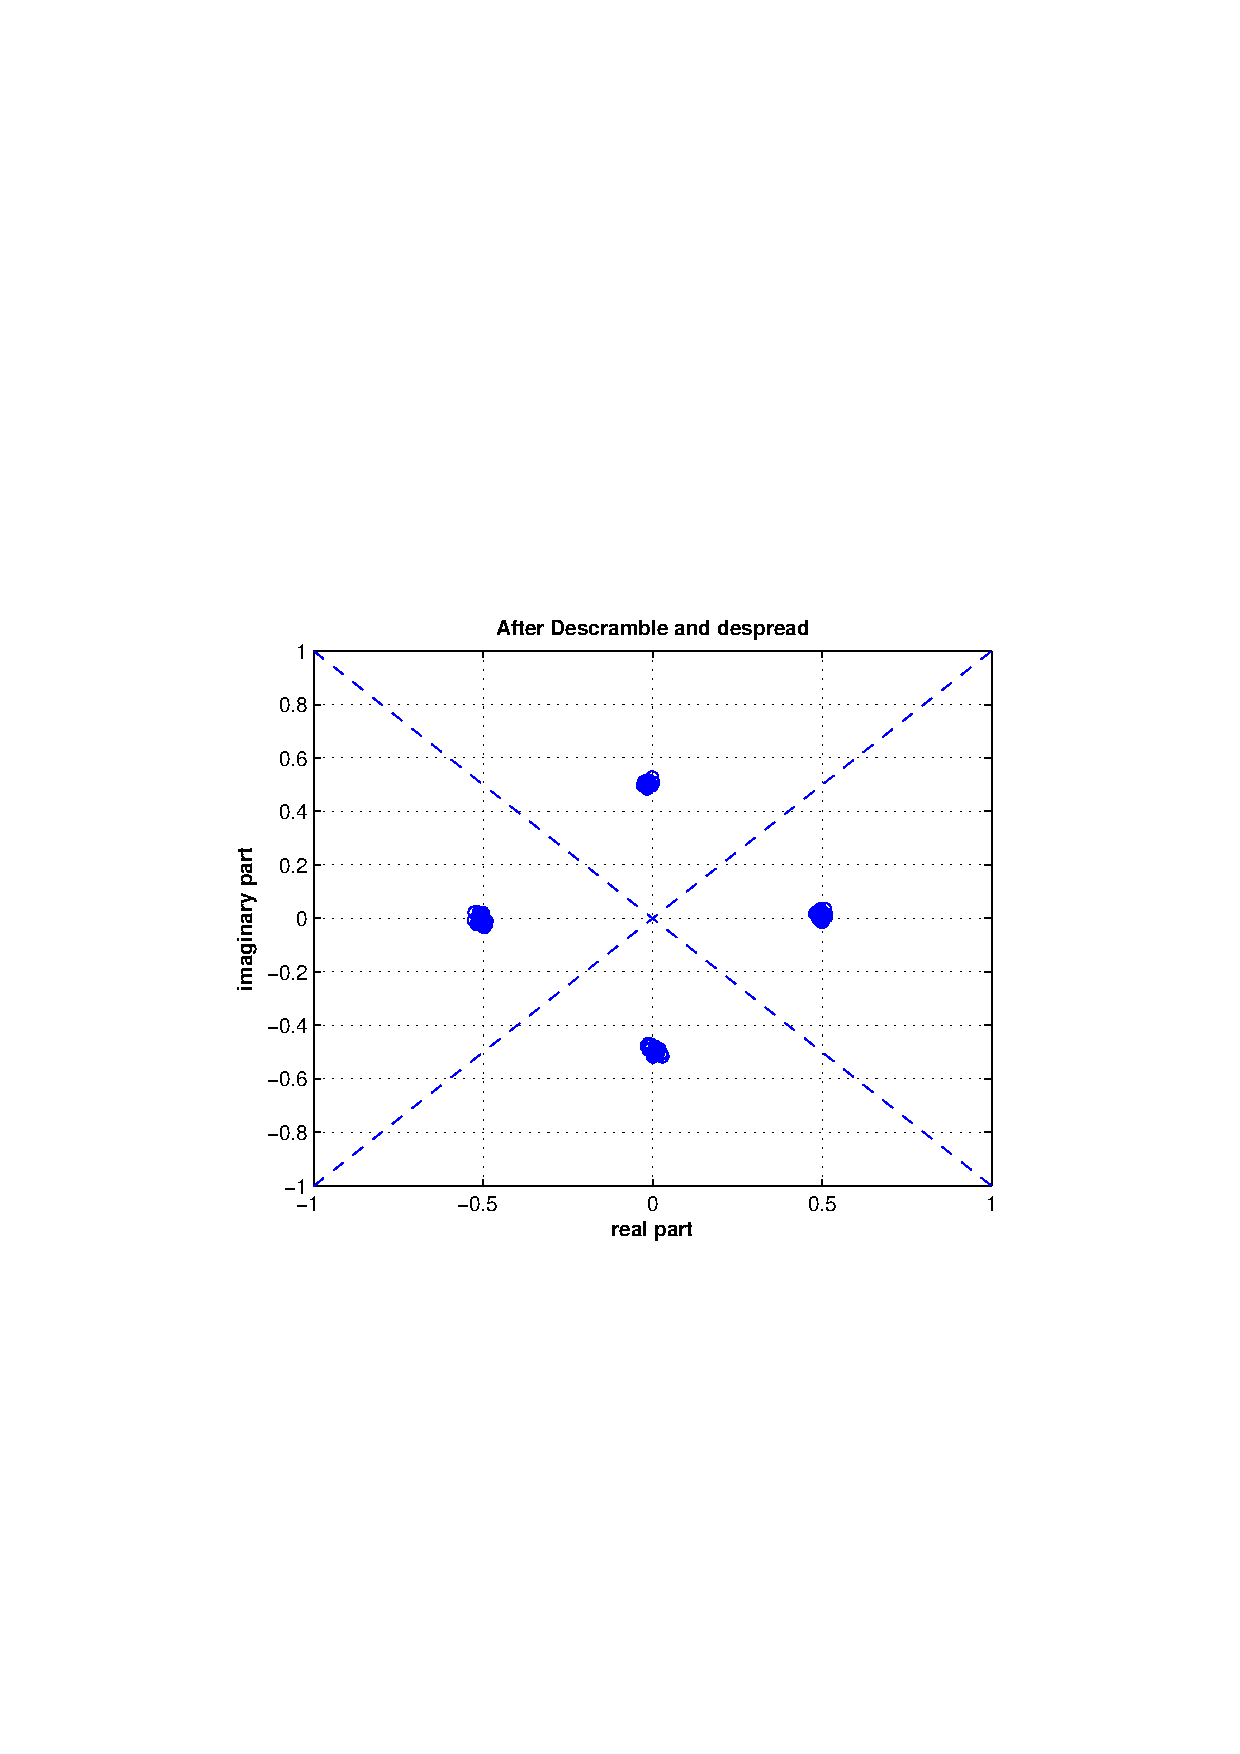
\includegraphics[width=3in]{ex1/afterDespread.pdf} }
	\end{center}
	\caption{Complex signal after descramble or despread}
	\label{fig:descrAdespr}
\end{figure}

\section{Summary}
From the symbol error checking after the decide function we get no error in our experiment. In other words, in our experiment environment we can achieve an error free transmission. From this first exercise we have a general idea of how a single CDMA Signal is transmitted in the wireless channel, what is the basic procedure of signal processing in UMTS (eg. descrambling and despreading). Meanwhile we realize the importance of frame synchronization in wireless communication (in our case, we first try to find the Imax to identify the frame start). In order to guarantee the accurate detection of data symbols, an oversampling is also a requirement in our experiment.